\chapter{Perancangan}
\label{chap:perancangan}

\section{Struktur Modul}
\label{sec:struktur_modul}
Berdasarkan fitur-fitur yang ada pada \textit{website} penyedia surat akademik, maka dirancang struktur modul yang menjelaskan mengenai modul-modul apa saja yang akan dirancang untuk membangun \textit{website} penyedia surat akademik. Garis besar dari struktur modul ini terbagi menjadi 3 bagian berdasarkan penggunanya, yaitu modul mahasiswa, modul TU dan modul pejabat.\
Gambar \hyperlink{struktur_modul_garis_besar}{4.1} menjelaskan struktur modul secara garis besar.



Selanjutnya, modul-modul yang telah disebutkan sebelumnya memiliki struktur tersendiri yang lebih spesifik. Gambar \hyperlink{struktur_modul_mahasiswa}{4.2} menjelaskan struktur modul mahasiswa secara menyeluruh.



Berdasarkan gambar di atas, berikut ini adalah penjelasan mengenai struktur modul mahasiswa dari \textit{\textit{website}} penyedia surat akademik :
\begin{enumerate}
	\item Modul \textit{login}.
	\item Modul buat surat.
	\item Modul cek riwayat pembuatan surat.
\end{enumerate}

Gambar \hyperlink{struktur_modul_tu}{4.3} menjelaskan struktur modul TU secara menyeluruh.

%\begin{figure}[H]
%	\centering
%		\includegraphics{}
%		\caption{Struktur modul TU}
%		\label{fig:struktur_modul_tu}
%\end{figure}

Berdasarkan gambar di atas, berikut ini adalah penjelasan mengenai struktur modul TU dari \textit{\textit{website}} penyedia surat akademik :
\begin{enumerate}
	\item Modul \textit{login}.
	\item Modul data mahasiswa.
	\item Modul format surat.
	\item Modul cek riwayat seluruh pembuatan surat.
\end{enumerate}

Gambar \hyperlink{struktur_modul_pejabat}{4.4} menjelaskan struktur modul pejabat secara menyeluruh.

%\begin{figure}[h]
%	\centering
%		\includegraphics{}
%		\caption{Struktur modul pejabat}
%		\label{fig:struktur_modul_pejabat}
%\end{figure}

Berdasarkan gambar di atas, berikut ini adalah penjelasan mengenai struktur modul pejabat dari \textit{\textit{website}} penyedia surat akademik :
\begin{enumerate}
	\item Modul \textit{login}.
	\item Modul cek riwayat seluruh pembuatan surat.
\end{enumerate}

\section{Perancangan Fisik Basis Data}
\label{sec:perancangan_fisik_basis_data}
Berdasarkan diagram ER yang telah dibuat pada bab III, dapat dibangun perancangan fisik dari basis data untuk mengimplementasikan hubungan antar entitas.\

Tabel berikut ini menjelaskan entitas apa saja yang dibangun beserta dengan atribut-atribut pada entitas tersebut.

\begin{table}[H]
\centering
\caption{Tabel Entitas Mahasiswa}
\label{entitas_mahasiswa}
\begin{tabular}{|l|l|l|l|l|l|}
\hline
\textbf{Nama Field}&\textbf{Tipe Data}&\textbf{Panjang}&\textbf{Ket.}&\textbf{Null?}&\textbf{FK ke Relasi Lain}\\ \hline
NIRM&varchar&255&&Not null&\\ \hline
NPM&varchar&255&&Not null&\\ \hline
Nama&varchar&255&&Not null&\\ \hline
Jurusan&int&11&FK&Not null&Jurusan\\ \hline
Fakultas&int&11&FK&Not null&Fakultas\\ \hline
Angkatan&int&11&&Not null&\\ \hline
Kota lahir&varchar&255&&Not null&\\ \hline
Tanggal lahir&date&&&Not null&\\ \hline
Foto&varchar&255&&Not null&\\ \hline
Dosen wali&int&11&FK&Not null&Dosen\\ \hline
Username&varchar&255&&Not null&\\ \hline
Password&varchar&255&&Not null&\\ \hline
\end{tabular}
\end{table}

\begin{table}[H]
\centering
\caption{Tabel Entitas Dosen}
\label{entitas_dosen}
\begin{tabular}{|l|l|l|l|l|l|}
\hline
\textbf{Nama Field}&\textbf{Tipe Data}&\textbf{Panjang}&\textbf{Ket.}&\textbf{Null?}&\textbf{FK ke Relasi Lain}\\ \hline
NIK&varchar&255&&Not null&\\ \hline
Nama&varchar&255&&Not null&\\ \hline
Jurusan&int&11&FK&Not null&Jurusan\\ \hline
Fakultas&int&11&FK&Not null&Fakultas\\ \hline
Foto&varchar&255&&Not null&\\ \hline
Username&varchar&255&&Not null&\\ \hline
Password&varchar&255&&Not null&\\ \hline
\end{tabular}
\end{table}

\begin{table}[H]
\centering
\caption{Tabel Entitas Mata Kuliah}
\label{entitas_mata_kuliah}
\begin{tabular}{|l|l|l|l|l|l|}
\hline
\textbf{Nama Field}&\textbf{Tipe Data}&\textbf{Panjang}&\textbf{Ket.}&\textbf{Null?}&\textbf{FK ke Relasi Lain}\\ \hline
Kode matkul&varchar&255&&Not null&\\ \hline
Nama&varchar&255&&Not null&\\ \hline
Jurusan&int&11&FK&Not null&Jurusan\\ \hline
Sks&int&11&&Not null&\\ \hline
\end{tabular}
\end{table}

\begin{table}[H]
\centering
\caption{Tabel Entitas Jurusan}
\label{entitas_jurusan}
\begin{tabular}{|l|l|l|l|l|l|}
\hline
\textbf{Nama Field}&\textbf{Tipe Data}&\textbf{Panjang}&\textbf{Ket.}&\textbf{Null?}&\textbf{FK ke Relasi Lain}\\ \hline
Kode jurusan&varchar&255&&Not null&\\ \hline
Nama&varchar&255&&Not null&\\ \hline
Ketua jurusan&int&11&FK&Not null&Dosen\\ \hline
\end{tabular}
\end{table}

\begin{table}[H]
\centering
\caption{Tabel Entitas Fakultas}
\label{entitas_fakultas}
\begin{tabular}{|l|l|l|l|l|l|}
\hline
\textbf{Nama Field}&\textbf{Tipe Data}&\textbf{Panjang}&\textbf{Ket.}&\textbf{Null?}&\textbf{FK ke Relasi Lain}\\ \hline
Kode fakultas&varchar&255&&Not null&\\ \hline
Nama&varchar&255&&Not null&\\ \hline
Dekan&int&11&FK&Not null&Dosen\\ \hline
Wakil dekan I&int&11&FK&Not null&Dosen\\ \hline
Wakil dekan II&int&11&FK&Not null&Dosen\\ \hline
\end{tabular}
\end{table}

\begin{table}[H]
\centering
\caption{Tabel Entitas Format Surat}
\label{entitas_format_surat}
\begin{tabular}{|l|l|l|l|l|l|}
\hline
\textbf{Nama Field}&\textbf{Tipe Data}&\textbf{Panjang}&\textbf{Ket.}&\textbf{Null?}&\textbf{FK ke Relasi Lain}\\ \hline
Id format&varchar&255&&Not null&\\ \hline
Jenis surat&varchar&255&&Not null&\\ \hline
Ket.&varchar&255&&Not null&\\ \hline
Link format&varchar&255&&Not null&\\ \hline
\end{tabular}
\end{table}

\begin{table}[H]
\centering
\caption{Tabel Entitas Pesanan Surat}
\label{entitas_pesanan_surat}
\begin{tabular}{|l|l|l|l|l|l|}
\hline
\textbf{Nama Field}&\textbf{Tipe Data}&\textbf{Panjang}&\textbf{Ket.}&\textbf{Null?}&\textbf{FK ke Relasi Lain}\\ \hline
Id&int&10&PK&Not null&\\ \hline
Tanggal buat&timestamp&255&&Not null&\\ \hline
Pemohon&int&11&FK&Not null&Mahasiswa\\ \hline
Jenis surat&int&11&FK&Not null&Format surat\\ \hline
Data surat&text&65,535&&Not null&\\ \hline
Penerima surat&varchar&255&&Not null&\\ \hline
Persetujuan dosen wali&tinyint&1&&Not null&\\ \hline
Persetujuan Kaprodi&tinyint&1&FK&Not null&Dosen\\ \hline
Persetujuan WD II&varchar&255&FK&Not null&Dosen\\ \hline
Persetujuan WD I&varchar&255&FK&Not null&Dosen\\ \hline
Persetujuan dekan&varchar&255&FK&Not null&Dosen\\ \hline
\end{tabular}
\end{table}

\begin{table}[H]
\centering
\caption{Tabel Entitas History Surat}
\label{entitas_history_surat}
\begin{tabular}{|l|l|l|l|l|l|}
\hline
\textbf{Nama Field}&\textbf{Tipe Data}&\textbf{Panjang}&\textbf{Ket.}&\textbf{Null?}&\textbf{FK ke Relasi Lain}\\ \hline
Nomor surat&varchar&255&&Not null&\\ \hline
Perihal&varchar&255&&Not null&\\ \hline
Penerima surat&varchar&255&&Not null&\\ \hline
Pemohon&int&11&FK&Not null&Mahasiswa\\ \hline
Jenis surat&int&11&FK&Not null&Format surat\\ \hline
Link arsip&varchar&255&&Not null&\\ \hline
Penandatanganan&tinyint&11&&Not null&\\ \hline
Pengambilan&tinyint&11&&Not null&\\ \hline
\end{tabular}
\end{table}

\begin{table}[H]
\centering
\caption{Tabel Entitas History Surat}
\label{entitas_history_surat}
\begin{tabular}{|l|l|l|l|l|l|}
\hline
\textbf{Nama Field}&\textbf{Tipe Data}&\textbf{Panjang}&\textbf{Ket.}&\textbf{Null?}&\textbf{FK ke Relasi Lain}\\ \hline
Id&int&10&PK&Not null&\\ \hline
Id Dosen&int&11&FK&Not null&Dosen\\ \hline
Id fakultas&int&11&FK&Not null&Fakultas\\ \hline
\end{tabular}
\end{table}

\section{Perancangan Antar Muka}
\label{sec:perancangan_antar_muka}
Berdasarkan struktur modul yang telah dijelaskan pada bagian sebelumnya, maka dirancang antar muka untuk memberikan tampilan pada setiap fitur yang terdapat pada \textit{website} penyedia surat akademik. Pada bagian sebelumnya telah disebutkan \textit{website} penyedia surat akademik memiliki 3 aktor utama yaitu mahasiswa, pejabat dan petugas TU. Masing-masing aktor ini memilik antar muka yang berbeda-beda sesuai dengan fitur yang dapat dijalankannya.

\subsection{Antar Muka Untuk Mahasiswa}
\label{sec:antar_muka_mahasiswa}
Berdasarkan strutur modul, mahasiswa dapat menjalankan 2 fungsi yaitu membuat surat dan melihat surat yang sudah pernah dibuat yang akan dijelaskan sebagai berikut :

\begin{enumerate}
	\item Membuat surat\\
	Untuk membuat surat mahasiswa perlu menekan menu "Buat Surat" pada \textit{navigation bar} untuk masuk ke halaman pemilihan kategori surat yang akan dibuat. Gambar menunjukkan halaman pilih kategori surat.
	\begin{figure}[H]
	\centering
		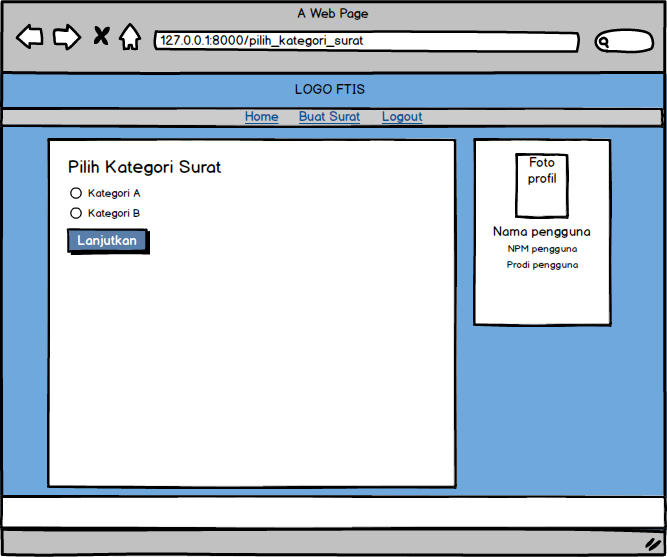
\includegraphics[scale=0.4]{F:/Skripsi/Template/Gambar/Mock_Up/Mahasiswa/pilih_kategori_surat.png}
		\caption{Pilih kategori surat}
		\label{fig:pilih_kategori_surat}
	\end{figure}
	
	Setelah memilih kategori surat mahasiswa akan diarahkan ke halaman selanjutnya untuk memilih jenis surat yang akan dibuat. Gambar menunjukkan halaman pilih jenis surat.
	\begin{figure}[H]
	\centering
		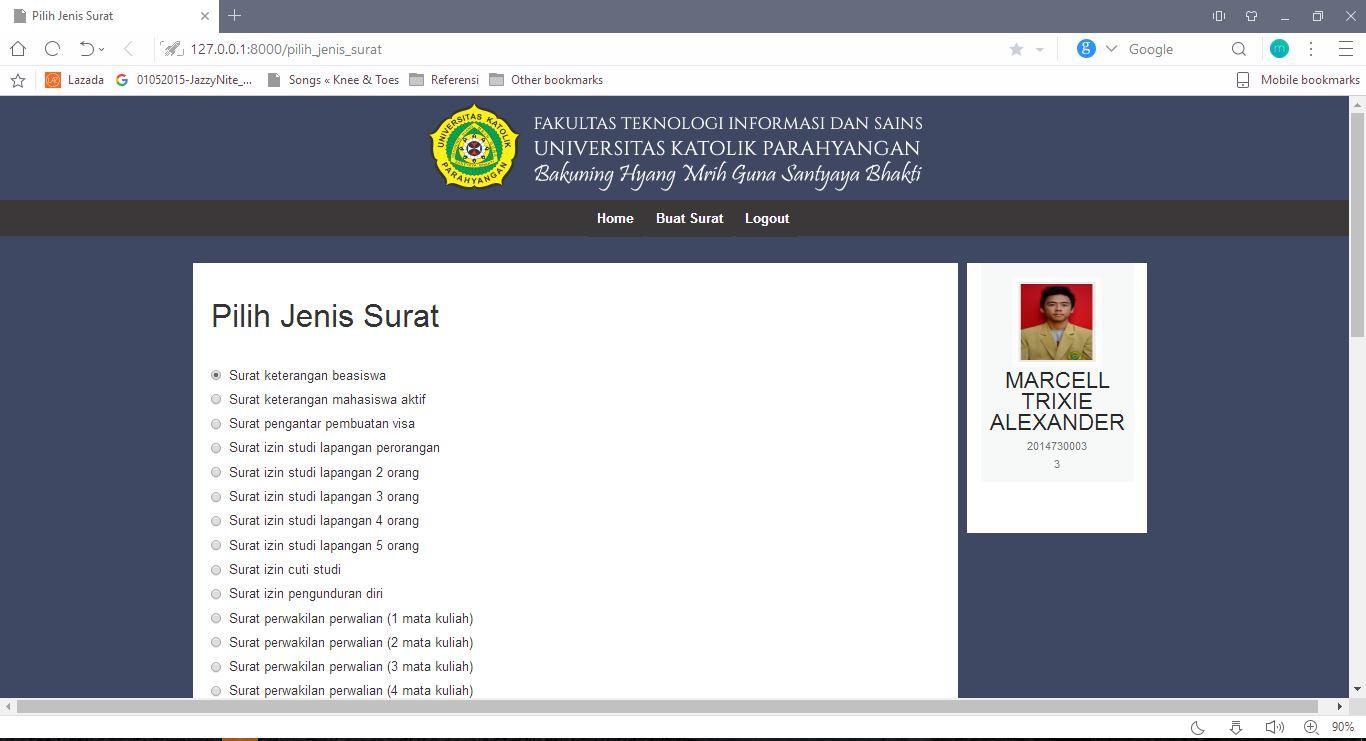
\includegraphics[scale=0.4]{F:/Skripsi/Template/Gambar/Mock_Up/Mahasiswa/pilih_jenis_surat.png}
		\caption{Pilih jenis surat}
		\label{fig:pilih_jenis_surat}
	\end{figure}
	
	Setelah memilih jenis surat mahasiswa akan diarahkan ke halaman selanjutnya yaitu halaman pengisian data surat. Gambar menunjukkan halaman pengisian data surat.
	\begin{figure}[H]
	\centering
		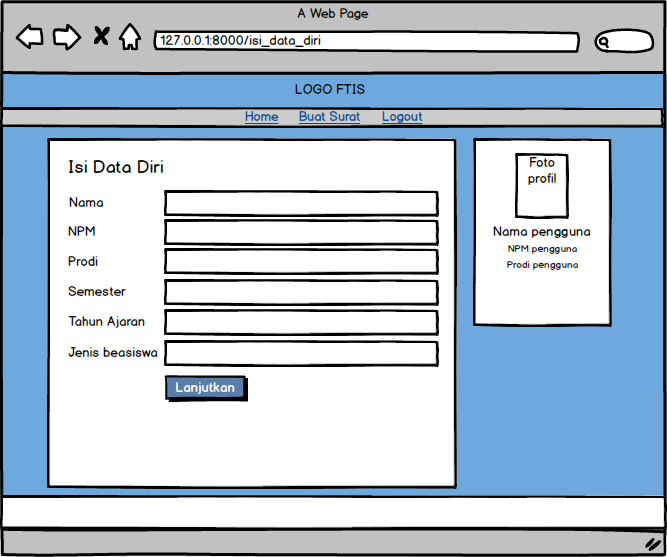
\includegraphics[scale=0.4]{F:/Skripsi/Template/Gambar/Mock_Up/Mahasiswa/pengisian_data.png}
		\caption{Contoh halaman pengisian data surat}
		\label{fig:contoh_halaman_pengisian_data_surat}
	\end{figure}
	
	Apabila semua data tela diisikan pada halaman pengisian data, mahasiswa akan diarahkan ke halaman selanjutnya untuk melihat apakah data isiannya sudah benar atau belum. Apabila data isian sudah benar mahasiswa dapat menekan tombol "Buat Surat", namun apabila ada data yang hendak diperbaiki mahasiswa dapat menekan tombol kembali. Gambar menunjukkan halaman \textit{preview} isi data surat.
	\begin{figure}[H]
	\centering
		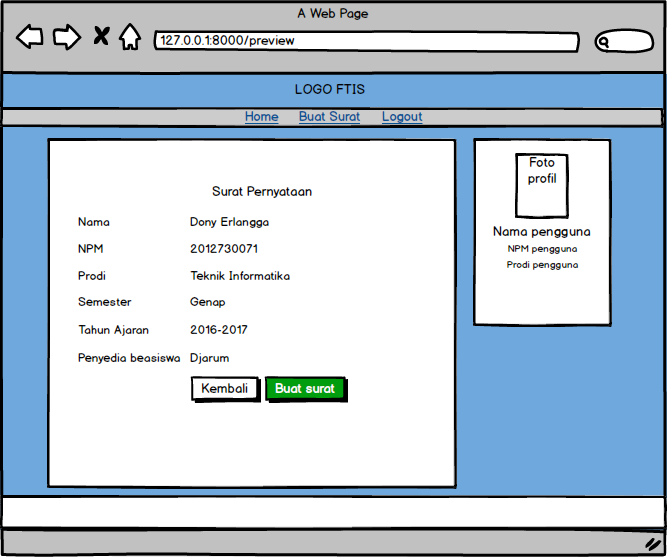
\includegraphics[scale=0.4]{F:/Skripsi/Template/Gambar/Mock_Up/Mahasiswa/preview_isian_data.png}
		\caption{Contoh halaman pengisian data surat}
		\label{fig:contoh_halaman_pengisian_data_surat}
	\end{figure}
	
	\item Melihat surat yang sudah pernah dibuat\\
	Surat-surat yang pernah dibuat oleh mahasiswa ybs. akan ditampilkan pada halaman \textit{home mahasiswa}. Gambar menunjukkan halaman \textit{home mahasiswa} yang menampilkan surat yang sudah pernah dibuat.

	\begin{figure}[H]
	\centering
		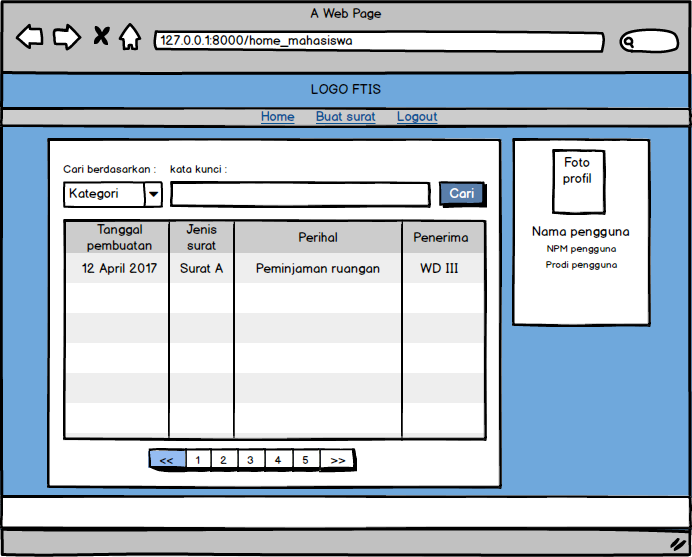
\includegraphics[scale=0.4]{F:/Skripsi/Template/Gambar/Mock_Up/Mahasiswa/home_mahasiswa.png}
		\caption{Home mahasiswa yang pernah membuat surat}
		\label{fig:home_mahasiswa_yang_pernah_membuat_surat}
	\end{figure}
	
	Apabila mahasiswa ybs. belum pernah membuat surat sekalipun, maka tampilan untuk halaman \textit{home mahasiswa} akan menampilkan seperti pada gambar berikut. Gambar menunjukkan halaman \textit{home mahasiswa} apabila mahasiswa ybs. belum pernah membuat surat.
	\begin{figure}[H]
	\centering
		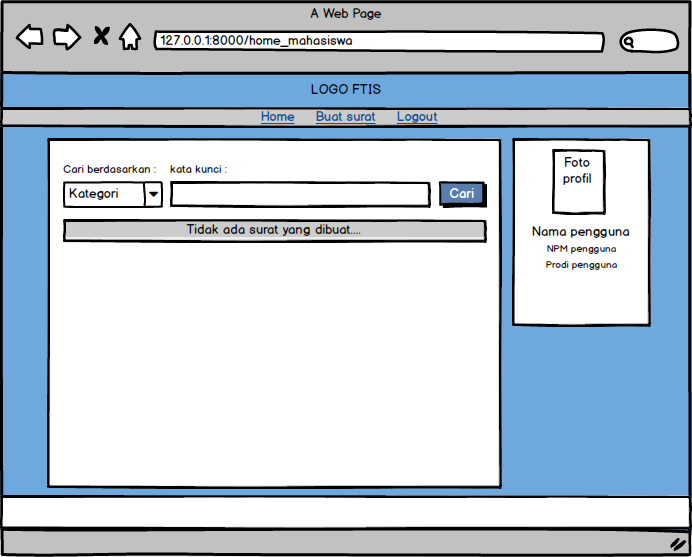
\includegraphics[scale=0.4]{F:/Skripsi/Template/Gambar/Mock_Up/Mahasiswa/home_mahasiswa_kosong.png}
		\caption{Home mahasiswa yang belum pernah membuat surat}
		\label{fig:home_mahasiswa_yang_belum_pernah_membuat_surat}
	\end{figure}
\end{enumerate}

\subsection{Antar Muka Untuk Pejabat}
\label{sec:antar_muka_pejabat}
Berdasarkan strutur modul, pejabat dapat menjalankan 3 fungsi yaitu melihat pesanan surat, menambahkan persetujuan dan catatan dan mengubah status penandatanganan surat yang sudah dibuat yang akan dijelaskan sebagai berikut :
\begin{enumerate}
	\item Melihat pesanan surat
	Surat-surat yang pernah dibuat oleh mahasiswa akan ditampilkan pada halaman \textit{home pejabat}. Gambar menunjukkan halaman \textit{home pejabat} yang menampilkan surat yang sudah pernah dibuat.
	\begin{figure}[H]
	\centering
		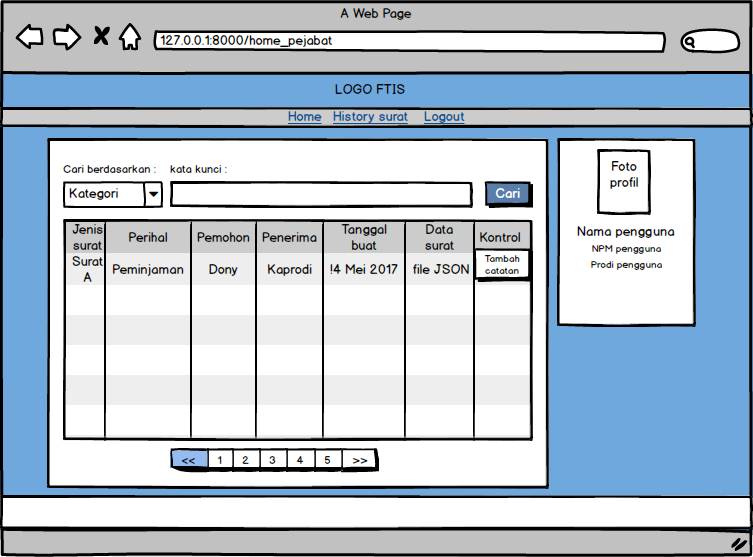
\includegraphics[scale=0.4]{F:/Skripsi/Template/Gambar/Mock_Up/Pejabat/home_pejabat.png}
		\caption{Home mahasiswa yang pernah membuat surat}
		\label{fig:home_mahasiswa_yang_pernah_membuat_surat}
	\end{figure}
	
	\item Menambahkan persetujuan dan catatan
	Untuk menambahkan persetujuan dan catatan pejabat perlu masuk ke halaman \textit{home pejabat}. Pada pojok kanan tabel terdapat tombol "Tambah Catatan" yang apabila di tekan akan mengarahkan pejabat ke halaman pengisian persetujuan dan catatan.Gambar menunjukkan halaman \textit{home pejabat} yang menampilkan surat yang sudah pernah dibuat.
	\begin{figure}[H]
	\centering
		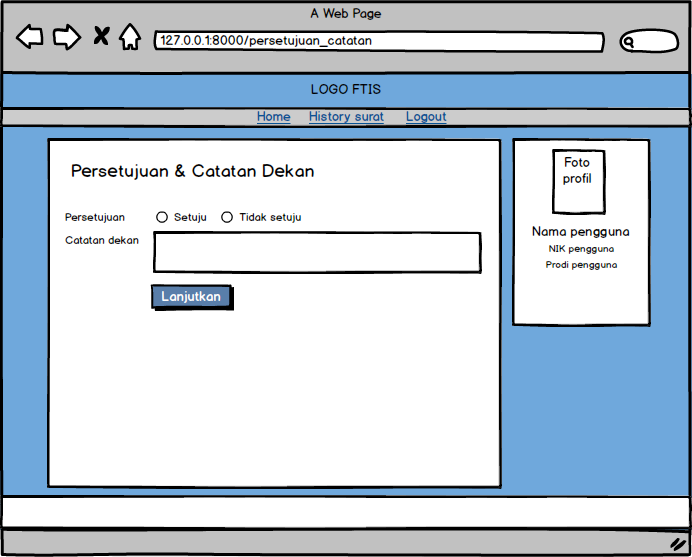
\includegraphics[scale=0.4]{F:/Skripsi/Template/Gambar/Mock_Up/Pejabat/persetujuan_catatan.png}
		\caption{Home mahasiswa yang pernah membuat surat}
		\label{fig:home_mahasiswa_yang_pernah_membuat_surat}
	\end{figure}
	
	\item
\end{enumerate}
\subsection{Antar Muka Untuk Petugas TU}
\label{sec:antar_muka_petugas_tu}
Berdasarkan strutur modul, petugas TU dapat menjalankan 4 fungsi yaitu menambahkan nomor surat dan meng-\textit{generate} surat, menambahkan list data mahasiswa dan format surat baru dan mengubah status pengambilan surat yang sudah dibuat yang akan dijelaskan sebagai berikut :
\begin{enumerate}
	\item Menambahkan nomor surat dan meng-\textit{generate} surat
	\item menambahkan list data mahasiswa
	\item menambahkan format surat baru
	\item mengubah status pengambilan surat
\end{enumerate}